\section{Theorie}
\label{sec:Theorie}

Laserstrahlen sind elektromagnetische Wellen, die sich von üblichen Lichtquellen durch eine viel höhere Intensität mit fast monochromatischem Licht und einer großen Kohärenzlänge unterscheidet.\\
Sie werden in einer Laserapparatur, die aus drei Hauptbestandteilen zusammengesetzt ist, erzeugt. Ein aktives und ein Pumpmedium erzeugen den Strahl, der von zwei Spiegeln, die den Resonator bilden, zum einen total und zum anderen teilreflektiert werden und dadurch eine hohe Verstärkung ermöglichen. Die Medien können in allen klassichen Aggregatzuständen vorliegen, wobei in diesem Versuch ein Laser mit gasförmigen Medien betrachtet wird. Der Aufbau ist schematisch für einen Laser mit Helium als Pump- und Neon als aktivem Medium (He-Ne-Laser) in Abbildung \ref{fig:skizzeLaser} dargestellt.

\begin{figure}
  \centering
  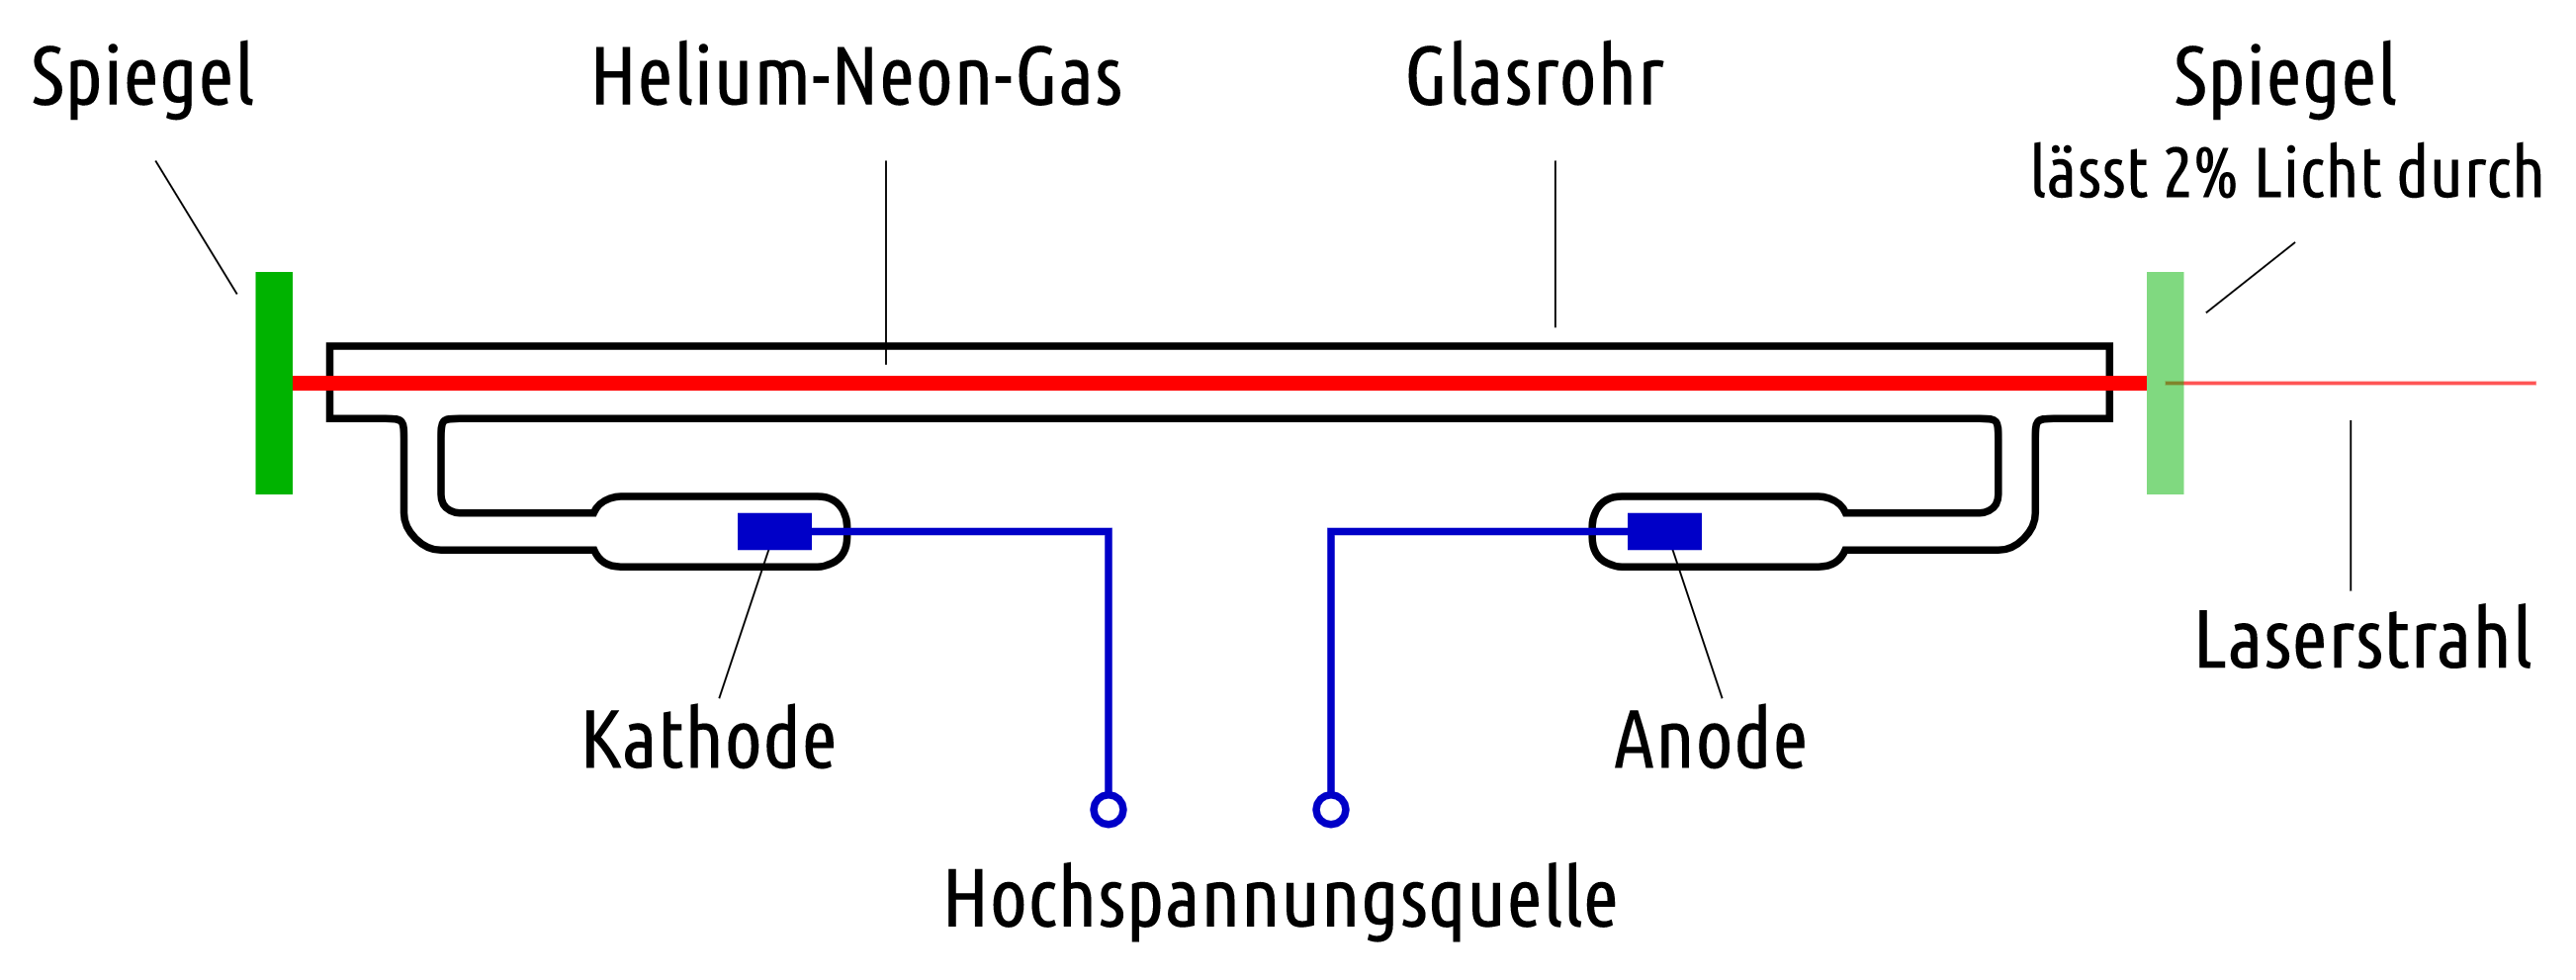
\includegraphics[width=\textwidth]{data/apparatur.png}
  \caption{Darstellung einer Laserappatur für Helium und Neon als Medien.\cite{leifi}}
  \label{fig:skizzeLaser}
\end{figure}

\subsection{Erzeugung von Laserlicht}
\label{sec:erzeugung}
Die Vorgänge bei der Erzeugung von Laserlicht basieren auf drei Wechselwirkungen von Photonen, also elektromagnetischer Strahlung, und den Elektronen in Atomen, die auf diskrete Energieniveaus aufgeteilt sind. Die drei Möglichkeiten sind in Abbildung \ref{fig:mechanismenStrahlung} skizziert.

\begin{figure}
  \centering
  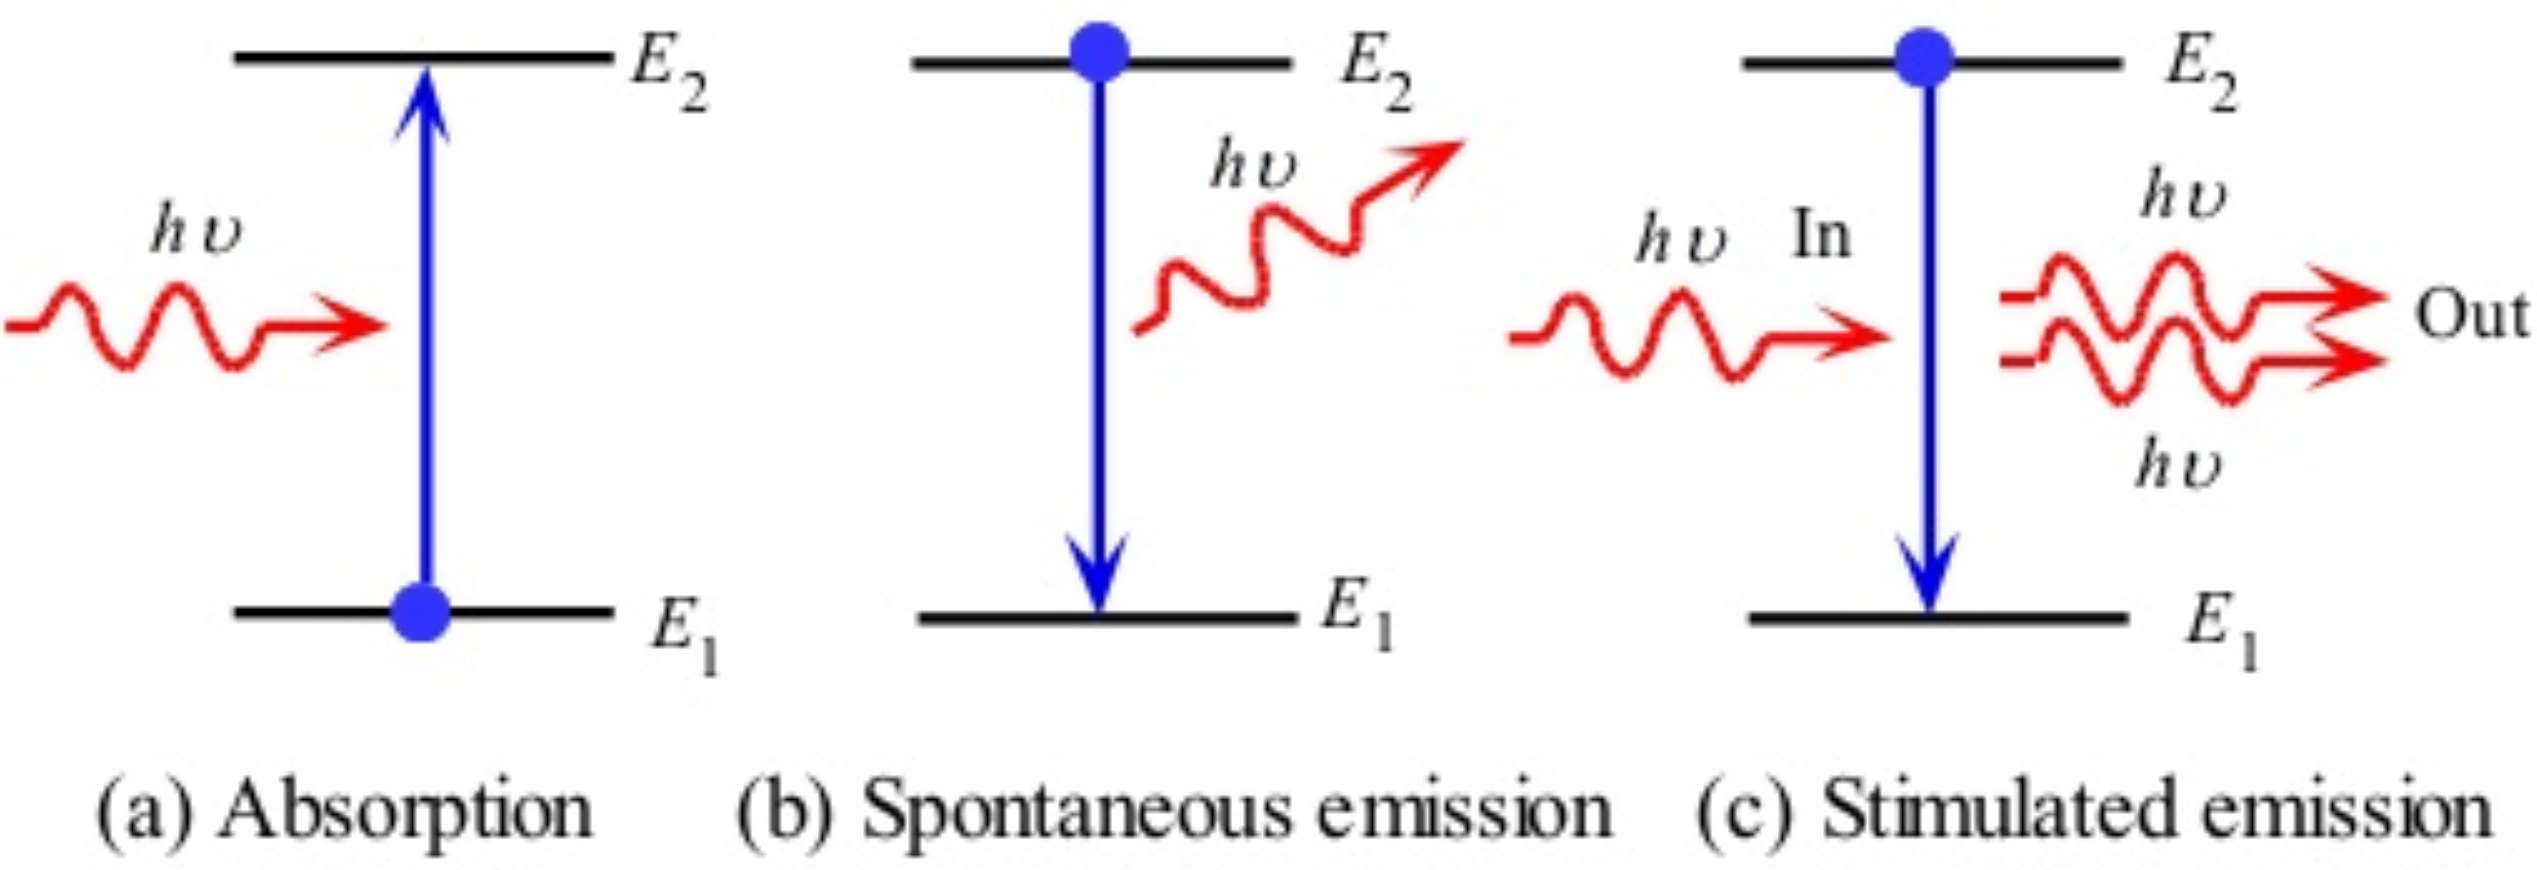
\includegraphics[width=\textwidth]{data/mechanismenStrahlung.png}
  %https://going-postal.com/2017/11/how-does-a-laser-work/pic-01-2/
  \caption{Darstellung der drei fundamentalen Strahlungs-Materie-Wechselwirkungen für die Erzeugung von Laserlicht.\cite{goingPostal}}
  \label{fig:mechanismenStrahlung}
\end{figure}

Bei der Absorption wird ein Photon von einem Atom absorbiert. Dadurch wird ein Elektron von einem niederenergetischen Niveau auf ein höheres Niveau angehoben, seine Energie steigt und das Photon verschwindet. Dieser Prozess kann nur dann stattfinden, wenn das Photon ungefähr eine Energie hat, die der Energiedifferenz der Niveaus entspricht.\\
Die spontane Emission beschreibt das typische Zerfallen von angeregten Zustanden mit einer begrenzten Lebensdauer in Zustände, für die der Übergang erlaubt ist. Dabei wird ein Photon mit zufälliger Phase und Richtung ausgesandt. Seine Energie ist die Energiedifferenz zwischen den beiden Niveaus.\\
Bei der stimulierten Emission löst ein Photon mit der Energie der Energieniveaudifferenz den Zerfall aus. Dabei wird ein weiteres Photon ausgesandt, das dem einfallenden in Richtung, Energie und Phase gleicht. Die beiden Photonen sind somit kohärent.

Es ist ersichtlich, dass nur der Mechanismus der stimulierten Emission eine Möglichkeit bietet, Licht stark zu verstärken, um einen kohärenten, möglichst monochromatischen und nicht zerlaufenden Strahl zu erhalten. Dazu ist eine sogenannte Besetzungsinversion nötig. Die liegt dann vor, wenn ein Niveau oberhalb des Grundzustandes mehr als zur Hälfte gefüllt ist, wobei alle Atome im aktiven Medium betrachtet werden. Dies kann nie in einem Zweiniveausystem geschehen, weil dort die Energie für die Anregung gleich der Energie für die stimulierte Emission ist und diese Prozesse deswegen konkurrieren. Für einen funktionierenden Laser ist somit mindestens ein Dreiniveausystem nötig.\\
Dabei werden Elektronen aus dem Grundzustand in einen hoch angeregten Zustand gehoben. Dies geschieht beim He-Ne-Laser durch Stöße zweiter Art zwischen den Helium- und Neonatomen. Der Zustand zerfällt schnell in einen niedrigeren metastabilen Zustand mit (im Vergleich zum Mutterzustand) hoher Lebensdauer durch spontane Emission. Nun können Photonen mit der passenden Energie die stimulierte Emission hervorrufen und sich somit vervielfältigen. Anfängliche Photonen für diesen Prozess können zum Beispiel aus der spontanen Emission des metastabilen Zustands stammen.

Die Resonatorspiegel sind dafür verantwortlich, die Photonen aus der stimulierten Emission häufig genug erneut durch das aktive Medium gehen zu lassen, um eine Basis für die Besetzungsinversion zu haben. Nur ein geringer Teil der Photonen aus einem Durchlauf durch die Apparatur verlässt als scharfer Laserstrahl den Aufbau.
